%-----------------------------------------------------------------------------
%
%          PHYSICS  M.S.     THESIS
%          JUSTIN A. VASEL
%
%          This began as the template offered by the University of Minnesota, 
%          but I've made a few changes here and there...  
%
%          -->  supernovae.tex
%
%-----------------------------------------------------------------------------


\chapter{Neutrino Production in Supernovae}
	\label{supernovae_chapter}

	\vspace{-0.2in}

	\begin{quoting}
		\noindent \large ``Stars are phoenixes, rising from their own ashes." \normalsize

		--- Carl Sagan
	\end{quoting}

	\chapterIntro{S}{tars are like us: They are born. They live. They die. } A star's mass is its most telling feature. It determines how they live and how they die. Low-mass stars have cooler cores and lower rates of nuclear fusion. They expend their fuel very slowly and as a result tend to live long lives that last billions of years. They will often end their lives as a white dwarf; a dense ball of glowing degenerate matter that very slowly cools over time. High-mass stars have contrasting features. They are short-lived due to their rapid exhaustion of nuclear fuel, lasting only millions of years. And instead of fading away in the night sky at the end of their lives, massive stars go out with a bang. Their passing is marked by a brilliant explosion that can easily outshine an entire galaxy: the supernova.
	

	%% SECTION : SUPERNOVA TAXONOMY
	\section{Supernova Taxonomy}
		Supernova taxonomy is not an exact science. They are classified merely by the appearance of their spectra. In that respect, supernovae are to the astronomer as insects are to the biologist, rocks to the geologist, or artifacts to the archaeologist. The classification of supernovae is---as Ernest Rutherford would say---stamp collecting. 
		Generally speaking there are two types of supernova: Type I and Type II. The difference between them is that the spectra of Type II supernovae contain very prominent hydrogen lines, while those of Type I do not. Furthermore the Type I supernovae are divided into two types depending on whether their spectra contain silicon (Type Ia) or not. The latter of these---devoid of hydrogen and devoid of silicon---are again divided in two, depending on whether they're helium rich (Type Ib) or helium poor (Type Ic) (\FIG \ref{fig:sn_types}).

		Type Ia supernovae are perhaps the most distinct of the three Type I supernovae. The situation in which they are thought to occur is that of a white dwarf in binary orbit with a companion star. Matter from the companion accretes onto the white dwarf until the Chandrasekhar limit of \ 1.4 \emph{M}$_\odot$ is reached. At that point the degeneracy pressure is overcome by gravity, causing the white dwarf to collapse and then explode when its carbon ignites. The explosion is so catastrophic that there is likely no remnant left in its wake. What's interesting about Type Ia supernovae is that they all explode at the same mass, 1.4 \emph{M}$_\odot$. The consistency of their eruptions---and, therefore, their spectra---make them ideal standard candles, allowing the astronomer to calculate intergalactic distances simply by measuring the peak brightness of their light curve.

		Type Ib and Ic supernovae are products of massive stars that have shed their outer envelopes of hydrogen and possibly helium. They explode via ``core-collapse'' and leave behind a neutron star or a black hole in their wake, generating a wealth of neutrinos in the process. 

		The Type II supernovae are also divided into two groups and are distinguished by the shape of their light curve. The Type II-L has a light curve that decays rather linearly after maximum brightness while the Type II-P has one that plateaus after maximum brightness. Stars that become Type II supernovae are massive. As a result, they tend to live relatively short lives, making them more likely to be found in the arms of spiral galaxies where active star formation is occurring. The explosion mechanism for Type II supernovae is core-collapse, like the Type Ib/Ic supernovae. 
		These Type II supernovae are more common\cite{sn_rate} and will be the focus of the rest of the chapter. Throughout the rest of this thesis, I will make no further distinction between the Type II and Type Ib/Ic supernovae, but will instead refer to them collectively as ``core-collapse'' supernovae.

		\begin{figure}[H]
			\begin{center}
				\begin{tikzpicture}[every path/.style={>=latex}, type/.style={draw,rectangle,fill=red!20,anchor=west}]
				  \node[type] 	(SN) at (0,0) {SN};
				  \node[type]     (i) at (3,2.25)  { Type I};
				  \node[type] 	(ii) at (3,-2.25) { Type II};

				  \node[type] 	(ia) at (11,3) { Type Ia};
				  \node[type] 	(ibc) at (7,0.75) { Type Ib,Ic};
				  \node[type] 	(ib) at (11,1.5) { Type Ib};
				  \node[type] 	(ic) at (11,0) { Type Ic};

				  \node[type] 	(iil) at (11,-1.5) { Type II-L};
				  \node[type] 	(iip) at (11,-3) { Type II-P};

				  \draw[->] (SN) edge node[sloped, anchor=center, above, text width=1.0cm] {\color{light-gray} \footnotesize no H}(i);
				  \draw[->] (SN) edge node[sloped, anchor=center, below, text width=0.8cm] {\color{light-gray} \footnotesize H}(ii);
				  \draw[->] (i)  edge node[sloped, anchor=center, above, text width=0.8cm] {\color{light-gray} \footnotesize Si}(ia);
				  \draw[->] (i)  edge node[sloped, anchor=center, below, text width=1.0cm] {\color{light-gray} \footnotesize no Si}(ibc);
				  \draw[->] (ibc)  edge node[sloped, anchor=center, above, text width=1.0cm] {\color{light-gray} \footnotesize He}(ib);
				  \draw[->] (ibc)  edge node[sloped, anchor=center, below, text width=1.0cm] {\color{light-gray} \footnotesize no He}(ic);
				  \draw[->] (ii)  edge node[sloped, anchor=center, above, text width=0.8cm] {\color{light-gray} \footnotesize Linear}(iil);
				  \draw[->] (ii)  edge node[sloped, anchor=center, below, text width=0.8cm] {\color{light-gray} \footnotesize Plateau}(iip);
				\end{tikzpicture}
			\end{center}
			\caption[Classification of Supernovae]{\bf Classification of supernovae. \rm All except for Type Ia are core-collapse supernovae. Neutrinos are produced in great quantities during core-collapse.} \label{fig:sn_types}
		\end{figure}


	%% SECTION : SHELL BURNING
	\section{Shell Burning}
		Stars of mass \emph{M} $\gtrsim$ 8 \emph{M}$_\odot$ undergo a relatively brief period at the end of their lives in which a series of nuclear reactions occur within their core\cite{bob}. When the hydrogen fuel is exhausted, the core contracts until the temperature is high enough to fuse helium. Once helium is exhausted, the core contracts again until carbon-burning begins. This process continues, the core burns through successively heavier elements, and the duration of each burning stage decreases substantially. The specifics of this process depend intimately on the mass of the star. An example for a 15 \emph{M}$_\odot$ star is summarized in \TAB \nolinebreak \ref{table:shell_burning}.

		\begin{table}[H]
		\centering
		\caption[Shell Burning Process for a 15 \emph{M}$_\odot$ Star]{\bf Shell Burning Process for a 15 \emph{M}$_\odot$ Star\rm\cite{Woosley2006}. Neutrino luminosity grows rapidly at each burning stage starting at carbon. }
		\label{table:shell_burning}
			\begin{tabular}{lcllccc}
				\toprule
				Stage & Time & Fuel & Main & Temp. & Density & Neutrino Loss\\
				 & Scale & & Product & (\SI{e9}{\kelvin}) & (\si{\gram\per\cubic\centi\metre}) & (Solar units) \\
				\midrule
				Hydrogen & 11 My & H & He & 0.035 & 5.8 & 1,800 \\
				Helium & 2 My & He & C, O & 0.18 & 1,390 & 1,900 \\
				Carbon & 2,000 y & C & Ne, Mg & 0.81 & \num{2.8e5} & \num{3.7e5} \\
				Neon & 0.7 y & Ne & O, Mg & 1.6 & \num{1.2e6} & \num{1.4e8} \\
				Oxygen & 2.6 y & O, Mg & Si, S & 1.9 & \num{8.8e6} & \num{9.1e8} \\
				Silicon & 18 d & Si, S & Fe, Ni & 3.3 & \num{4.8e7} & \num{1.3e11} \\
				Core collapse & $\sim$1 s & Fe & Neutron& $>7.1$ & $>$ \num{7.3e9} & $>$ \num{3.6e15} \\
				& & & Star & & & \\
				\bottomrule
			\end{tabular}
		\end{table}
		\vspace{-0.1in}
		The nuclear burning history of this process is contained within shells of unspent fuel that surround the core, producing a characteristic onion-like structure of progressively heavier elements. As the star burns through successively heavier nuclei, the mass and density of the core increases, driving up the temperature. Such high temperatures support the core by allowing it to fuse heavier nuclei, releasing nuclear binding energy. Simultaneously, the production and emission of neutrinos is a substantial source of energy loss for massive stars\cite{Woosley2006,astrophysics,Burrows2013,Janka2012}. Neutrino emission increases considerably after helium-burning, as seen in \TAB \ref{table:shell_burning}.\footnote{These neutrinos are not currently detectable at Earth; their energies and luminosities are too low.} At this point, the core and the stellar photosphere become decoupled; they are no longer connected by a mutual radiative transfer of energy.

		This emission is known as ``neutrino cooling''\footnote{This is also referred to as ``deleptonization'' because the only leptons present in a star---electrons and positrons---are transformed into neutrinos that promptly leave the star. The effect is a net deficit of leptons.} and consequentially accelerates the evolution of the star. The processes responsible for neutrino cooling are pair annihilation and the photoneutrino process\cite{astrophysics}:
		\begin{align}
			\text{pair annihilation:} \qquad &\HepProcess{\HepParticle{\Pelectron}{}{} + \HepParticle{\Ppositron}{}{} \HepTo \HepParticle{\Pnu}{}{} + \HepParticle{\APnu}{}{}} \label{eq:pairkill} \\
			\text{photoneutrino process:} \qquad &\HepProcess{\HepParticle{\Pphoton}{}{} + \HepParticle{\Pelectron}{}{} \HepTo \HepParticle{\Pelectron}{}{} + \HepParticle{\Pnu}{}{} + \HepParticle{\APnu}{}{}}
		\end{align}
		Pair annihilation occurs when the core temperature reaches $T_{core} \sim \SI{e9}{\kelvin}$\cite{Janka2012}. At this temperature high-energy photons undergo pair production, creating a wealth of free electrons and positrons. When they recombine they often produce more photons, but on rare occasions the interaction results in a neutrino-antineutrino pair instead. The photoneutrino process is much like Compton scattering, but instead the photon is transformed into a neutrino-antineutrino pair coming out of the interaction. 

		The net effect of neutrino cooling is essentially to move the progenitor core through the shell burning stages faster, and to drive the core mass to a limiting value known as the Chandrasekhar mass:
		\begin{equation}
			M_{\text{Ch}} = 5.84 \ Y^2_e \ M_\odot \approx 1.4 \ M_\odot
		\end{equation}
		where $Y_e$ is the number of electrons per nucleon. As the neutrinos stream from the core, they take energy with them leading to a steady reduction of entropy---and therefore an increase in electron degeneracy---in the core\cite{Burrows2013}. This exodus of neutrinos intensifies with each stage of nuclear burning, such that by the time the core is burning silicon, neutrino emission is enormous: A 20 $M_\odot$ star would have a photon luminosity of $\sim \SI[mode=text]{4.4e38}{ergs \second^{-1}}$ and a neutrino luminosity of $\sim \SI[mode=text]{3.1e45}{ergs \second^{-1}}$\cite{astrophysics}. These neutrinos are not currently detectable at Earth; their energies are below the observational limits of today's neutrino observatories.

		The products of silicon burning are nuclei centered around the $^{56}_{26}$Fe peak. Subsequent nuclear fusion of iron does not release nuclear binding energy, so there is no radiation pressure to support the core. The entropy of the core at this stage is very low ($\sim 0.7$ --- $1 \ k_b$ per nucleon\cite{Burrows2013})\footnote{$k_b$ is Boltzmann's constant.} and the electronic population is nearly fully degenerate and relativistic; the core briefly resembles a white dwarf. The only thing supporting the core is the electron degeneracy pressure, but with mass falling onto the iron core the Chandrasekhar mass is soon achieved and collapse proceeds unhindered.


	%% SECTION : CORE COLLAPSE
 	\section{Core Collapse}
		Two critical processes occur that are responsible for the iron core's collapse. The photodisintegration of iron nuclei (\EQ \ref{eq:photodis}) and electron capture on free protons (\EQ \ref{eq:ecapture}):
		\begin{align}
			\text{photodisintegration:} \qquad &\HepProcess{\HepParticle{\Pphoton}{}{} + ^{56}\text{Fe} \rightleftharpoons 13 \ ^{4}\text{He} + 4 \HepParticle{\Pneutron}{}{}} \label{eq:photodis}\\
			\text{electron capture:} \qquad & \HepProcess{\HepParticle{\Pelectron}{}{} + \HepParticle{\Pproton}{}{} \HepTo \HepParticle{\Pneutron}{}{} + \HepParticle{\Pnue}{}{}} \label{eq:ecapture}
		\end{align}
		Through photodisintegration, high-energy photons break apart iron nuclei into neutrons and alpha particles, effectively undoing the achievements of the star's multi-million-year lifetime. Cosmic tragedies aside, this process drives the collapse by consuming thermal energy and thus lowers the effective adiabatic index $\gamma$ at or below the critical value for gravitational stability of $4/3$\cite{astrophysics}.\footnote{Until now, $\gamma$ has remained at $5/3$, the typical value for a non-relativistic degenerate electron gas.}

		As the core begins to collapse, densities increase and so does the Fermi energy of the degenerate electrons. This allows them to capture on free protons (\EQ \ref{eq:ecapture}), reducing the number of electrons and accelerating the collapse. This process is widely known as ``neutronization.'' Electron neutrinos are produced in bulk in these reactions and can initially escape the collapse. However, the average energy of the neutrinos increases with density and temperature, and the cross section for coherent neutrino-nucleus scattering, 
		\begin{equation}
		\label{eq:nuScatXSection}
			\sigma \simeq 10^{-44} \ \text{cm}^2 \ N^2 \left(\frac{E_\nu}{\text{MeV}}\right)^2
		\end{equation}
		where $N$ is the number of neutrons in the nucleus, varies as the square of the neutrino energy. At a density $\rho_{\text{trap}} \simeq 10^{12}$ \si{\gram\per\cubic\centi\metre}, the in-falling material becomes opaque to neutrinos. The interface that separates neutrino-transparent regions from neutrino-opaque is known as the ``neutrinosphere
		'' and is analogous to the photosphere of a star. This trapping of neutrinos facilitates charged current interactions with the neutrons of nearby nuclei, the reverse process of \EQ \ref{eq:ecapture}. This balances the loss of electrons through the capture process and terminates the energy flow out of the core allowing the collapse to proceed adiabatically. The collapse continues all the way down to nuclear densities ($\rho \approx \SI{3e14}{\gram\per\cubic\centi\metre}$\cite{Janka2012,Janka2012a,particleastro}). The total time required for collapse from beginning to end is no more than $\sim\SI{350}{\milli\second}$ for any given progenitor\cite{Burrows2013}, during which the core's radius shrinks from $\sim \SI{3000}{\kilo\metre}$ to $\sim \SI{30}{\kilo\metre}$\cite{Woosley2006}.
	

	%% SECTION : REBOUND
	\section{Rebound}
		At nuclear densities, the nucleon degeneracy pressure halts the collapse. The inner core steepens and the in-falling material rebounds, producing a shock wave that moves outwards through the outer core. The shock wave begins in the neutrino-opaque region and moves into the neutrino-transparent region. As the shock front passes through the neutrinosphere the electron neutrinos are able to leave the star at once; an event known as ``neutrino breakout.'' The shock continues to heat up as it encounters the in-falling material, allowing the photodisintegration of iron to resume. This steals energy from the shock, and for stars with sufficiently massive iron cores, the shock will eventually stall before making it out of the core.

		Neutrinos play a key role in reviving the shock. The region outside the neutrinospheres\footnote{Each neutrino flavor has its own neutrinosphere. This is the case because the mean free path of a neutrino is related to its energy.} that surrounds the newly-formed proto neutron star is very hot and cools through the emission of neutrinos produced by electron capture and pair annihilation processes (\EQS \ref{eq:ecapture} \& \ref{eq:pairkill}). These neutrinos travel towards the shock front and eventually enter a dense region behind the shock where a small fraction of neutrinos are absorbed at a faster rate than they are emitted. This region occurs at a radius known as the ``gain radius,'' and gains thermal energy through neutrino heating. The deposited energy by the neutrinos is enough to revive the shock. The proto neutron star then gradually cools through neutrino emission.

		One expects the total radiated energy in a supernova explosion to be equal to the gravitational binding energy of the remnant neutron star. 
		\begin{equation}
			E_{rad} = \frac{3}{5} \frac{G M_{\text{ns}^2}}{R_{\text{ns}}} \approx \SI[mode=text]{e53}{ergs}
		\end{equation}
		Only $\sim 1\%$ of this energy manifests itself as electromagnetic radiation and kinetic energy of ejecta which produces the brilliant display that accompanies a supernova. The other $99\%$ is radiated away in the form of neutrinos.


	%% SECTION : SUPERNOVA NEUTRINO SPECTRA
	\section{Supernova Neutrino Spectra}
		Once neutrinos break out of the core, their motion is no longer diffusive like that of the photons and the shock wave. They are ejected into space before the outer layers of the star even ``know'' that the core has exploded. 
		\begin{figure}[H]
			\centering
			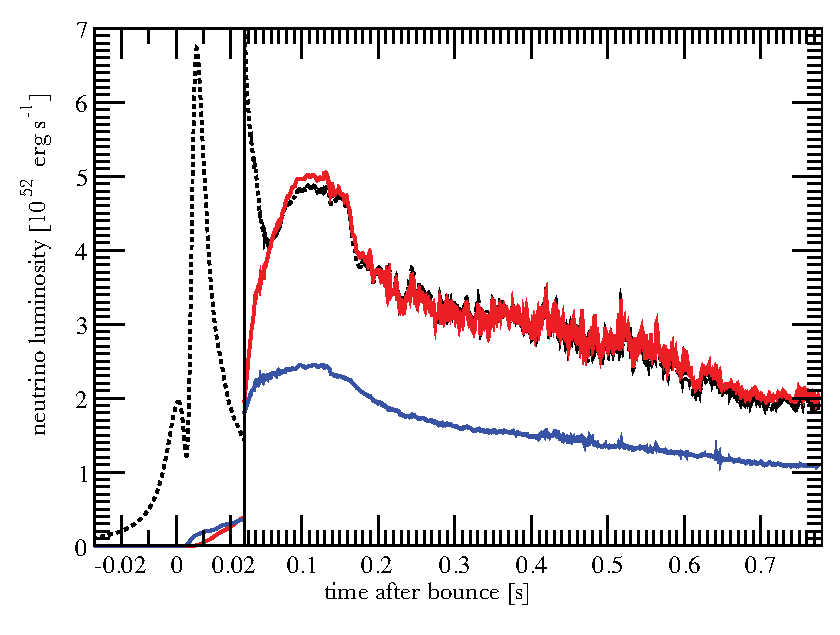
\includegraphics[width=0.8\textwidth]{neutrino_time}
			\caption[Simulated Supernova Neutrino Signal]{\bf Simulated supernova neutrino signal. \rm The simulation of this $15 M_\odot$ star was general relativistic and 2 dimensional. The black lines are for $\HepParticle{\Pnue}{}{}$, the red lines for $\HepParticle{\APnue}{}{}$, and the blue lines for heavier neutrinos $\nu_x$ \cite{Janka2012}. The neutrino flux persists for several tens of seconds and then fades.}
			\label{fig:neutrino_time}
		\end{figure}
		The electron neutrinos are the first to leave the star. These were the result of neutronization of the inner core and were the constituents of the neutrino breakout. This burst is expected to last for a few tens of milliseconds\cite{Scholberg2012}. Neutrinos generated during shock revival are also predominantly electron flavored. The duration of this period is on the order of $\sim\SI{100}{\milli\second}$\cite{Scholberg2012}. At a post-bounce time of $t \gtrsim\SI{100}{\milli\second}$, convective processes in the neutron star increase the flux of heavier neutrino flavors\cite{Janka2012a}. Over the next ten or twenty seconds, the core cools via neutrino emission (\FIG \ref{fig:neutrino_time}). The spectrum of neutrino energies (\FIG \ref{fig:neutrino_fluence}) emitted from the explosion are centered around a value just above \eMeV{10}\cite{cosmology}.

		\begin{figure}[H]
			\centering
			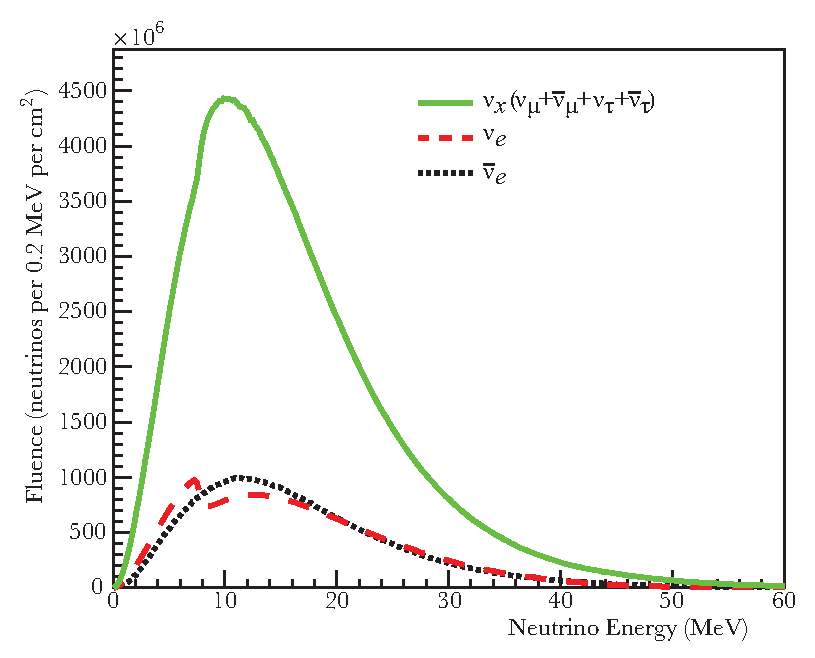
\includegraphics[width=0.9\textwidth]{neutrino_fluence}
			\caption[Simulated Supernova Neutrino Fluence]{\bf Simulated supernova neutrino fluence\rm \cite{Scholberg2012}. \rm The neutrino flux generated by the GVKM model\cite{Gava2009} for a supernova \SI{10}{\kilo\parsec} from Earth was integrated over a period of \SI{10}{\second} to produce this fluence. The energy distribution for all neutrino flavors are centered around $\gtrsim \eMeV{10}$. The model accounts for neutrino-neutrino interactions and dynamic MSW effects, which cause the wobble seen in the \HepParticle{\Pnue}{}{} profile.}
			\label{fig:neutrino_fluence}
		\end{figure}

		It is very helpful that $99\%$ of a supernova's energy is radiated in the form of neutrinos before the outer layers of the star are disrupted. This provides a means of predicting the optical appearance of a supernova. Such an advance warning would be invaluable to astronomy, as it would allow the community to observe a supernova as it happens and better understand the very complex process that surround it (see \CHP \ref{snews_chapter}). Furthermore, the neutrinos themselves can serve as more than just messengers; the properties of the neutrino flux would contain valuable insight to the goings-on in the core during and after collapse.

























%-----------------------------------------------------------------------------
%-----------------------------------------------------------------------------